\chapter{Multi-planar Reconstruction}
\vspace{-10mm}
\label{multiplanar}

Mult-planar Reconstruction (MPR) in medical imaging is a way of displaying three-dimensional images, captured on an imaging device. A three-dimensional study is displayed in three orthogonal slices. In each slice, there are indicated positions of the other two slices - each slice includes two lines giving the positions (See Figure \ref{fig:multiplanar}). The slices are most often parallel to basic anatomy planes\cite{ctteachingmanual}: sagittal, coronal and transverse plane.  Implementation of Multi-planar Reconstruction was requested by IKEM.

\begin{figure}
 	\caption{Multi-planar reconstruction in Dicom-Presenter.\label{fig:multiplanar}}
	\begin{center}
	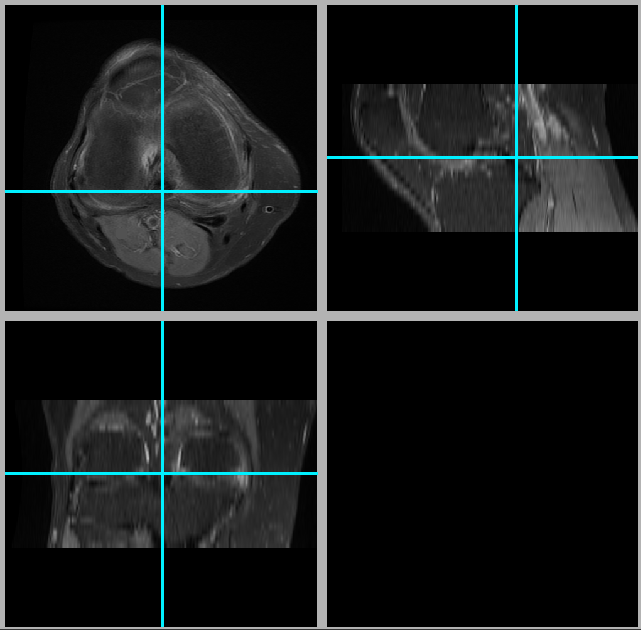
\includegraphics[width=0.75\textwidth]{Text/IMG/MultiPlanar.png}
	\end{center}
\end{figure}

\section{Implementation of Multi-planar Reconstruction}

An implementation of MPR could be divided into three parts:

\begin{itemize}
\item Handling user control. %User has to be able to freely manipulate with the three planes. Is existing
\item Image Rendering. %Is it possible to use existing classes to render three planes of a DICOM study?
\item Integration to existing object model. %The questions are, where to place the new class in the existing class hierarchy (see Section \ref{dpobjectmodel}) and how much functionality of the new class can be inherited from existing classes.
\end{itemize}

The question to discuss in all three steps is, how much of existing functionality can be used and what parts are nescessary to implemented. It is possible to implement a completely new class, which will handle user control and rendering itself. But it would lead to multiple implementations of similar tasks. The aim is to use maximum of existing functionality. There are few possible ways when creating a new class of how to try to use existing features:

\begin{itemize}
\item Modify existing class and create a new one.
\item Add new functionality into existing class.
\item Suggest a new class; abstract mutual features of some existing class and the suggested class to create a parent class, which will be inherited by both.
\end{itemize}
